\chapter{Machine learning for time series}
\label{cap:ml}

\section{What changes when data have an order}
Machine learning methods (random forests, boosting, neural networks) were designed, for the most part, for independent observations. In time series, three precautions are mandatory.

\subsection{Cross-validation that respects time}
Random cross-validation (shuffled \emph{k-fold}) mixes past and future. Since neighboring observations are similar, the model ``sees'' points almost identical to the one it is going to predict. This leaks information and understates the error.

\begin{simulacao}[Checked by simulation: leakage in validation]
A very persistent AR(1) series ($\phi=0.98$, noise with standard deviation 1), random forest with 5 lags as explanatory variables. RMSE with random cross-validation: $1.08$. RMSE with temporal validation (training on the past, testing on the future): $1.49$. The irreducible noise is $1.0$. The random procedure looks almost perfect. The temporal one shows the real performance, much worse. The difference is pure leakage.
\end{simulacao}

Always use \textbf{rolling or expanding window validation} (rolling origin, as in chapter~\ref{cap:prev}) and, when windows overlap, leave a gap between training and test.

\subsection{Trees do not extrapolate}
A tree (and a forest) predicts averages of observations already seen. If the series has a trend and the future leaves the training range, it gets ``stuck'' at the last level.

\begin{center}
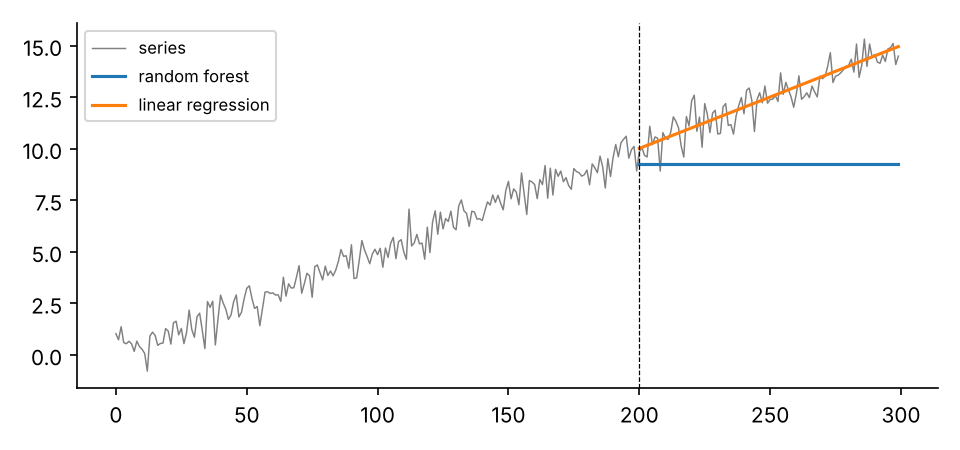
\includegraphics[width=0.75\textwidth]{fig/rf_extrapola.png}\\
\small A series with a linear trend. The random forest, trained up to $t=200$, predicts a flat level; linear regression continues the trend.
\end{center}

\begin{simulacao}
At the point $t=299$, the forest predicted $9.27$, and the value of the trend is $14.95$.
\end{simulacao}

Solutions: difference or detrend before fitting, model the change instead of the level, or use a hybrid model (linear trend plus forest on the residuals).

\subsection{Building the explanatory variables}
To turn forecasting into a regression problem: use lags ($y_{t-1},\dots,y_{t-p}$), moving averages, calendar variables (month, day of the week, holidays) and external regressors. Any statistic built with future data (for example, normalizing with the mean of the whole series) is leakage.

\section{Two useful families}
\begin{itemize}[leftmargin=1.4em]
\item \textbf{Global models}: instead of fitting one model per series, train a single model (for example, a recurrent neural network or boosting) with thousands of series. It helps when each series is short or noisy. It is the central idea of the Faloutsos et al.\ tutorial on large-scale forecasting.
\item \textbf{Time series classification}: the problem is not to forecast, but to assign a label to an entire series (for example, normal versus anomaly in an electrocardiogram). It is the focus of the \texttt{pyts} package, which offers techniques such as dynamic time warping, shapelets and image representations. Do not confuse it with forecasting.
\end{itemize}

\begin{atencao}[Pitfalls]
\begin{itemize}[leftmargin=1.2em]
\item \textbf{Always compare with the naive forecaster and with an ARIMA/ETS}. Many dazzling deep-network results disappear in front of a simple benchmark.
\item \textbf{Prediction intervals}: ML models give point forecasts. For uncertainty, use quantile regression, conformal prediction or simulation.
\item \textbf{Hyperparameters tuned on the test data}: the test set must be touched only once.
\end{itemize}
\end{atencao}

\begin{exercicio}
Why is shuffling the observations before splitting into training and test a mistake in a time series?
\end{exercicio}
\sol{Because it makes the model train on observations from the future and test on the past, and because adjacent observations are strongly dependent: test points have near-duplicates in training. The estimated error becomes unrealistically low. The correct test respects chronological order.}
